\documentclass[dvipdfmx,11pt,notheorems]{beamer}
%%%% 和文用 %%%%%
\usepackage{bxdpx-beamer}
\usepackage{pxjahyper}
\usepackage{minijs}%和文用
\usepackage{listings,jlisting} % プログラムの表示用
\usepackage{type1cm}
\renewcommand{\kanjifamilydefault}{\gtdefault}%和文用

%%%% スライドの見た目 %%%%%
\usetheme{Boadilla}
\usecolortheme{seahorse}
\usefonttheme{professionalfonts}
\setbeamertemplate{frametitle}[default][center]
\setbeamertemplate{navigation symbols}{}
\setbeamercovered{transparent}%好みに応じてどうぞ)
\setbeamertemplate{footline}[page number]
\setbeamerfont{footline}{size=\normalsize,series=\bfseries}
\setbeamercolor{footline}{fg=black,bg=black}

\setbeamercolor{white-cyan1}
{fg=white,bg=cyan!80!black}
\setbeamercolor{white-cyan2}
{fg=white,bg=cyan!60!black}

%フラットデザイン化
\setbeamertemplate{blocks}[rounded] % Blockの影を消す
%Beamer色設定
\definecolor{UniBlue}{RGB}{0,150,200}
\definecolor{AlertOrange}{RGB}{255,76,0}
\definecolor{AlmostBlack}{RGB}{38,38,38}
\setbeamercolor{structure}{fg=UniBlue} % 見出しカラー
\setbeamercolor{block title}{fg=UniBlue!50!black} % ブロック部分タイトルカラー
%%%%

%%%% 定義環境 %%%%%
\usepackage{amsmath,amssymb}
\usepackage{amsthm}
\usepackage{bm}
\theoremstyle{definition}
\newtheorem{theorem}{定理}
\newtheorem{definition}{定義}
\newtheorem{proposition}{命題}
\newtheorem{lemma}{補題}
\newtheorem{corollary}{系}
\newtheorem{conjecture}{予想}
\newtheorem*{remark}{Remark}
\renewcommand{\proofname}{}
%%%%%%%%%

%%%%% フォント基本設定 %%%%%
% \usepackage[T1]{fontenc}%8bit フォント
% \usepackage{textcomp}%欧文フォントの追加
% \usepackage[utf8]{inputenc}%文字コードをUTF-8
% \usepackage{otf}%otfパッケージ
% \usepackage{lxfonts}%数式・英文ローマン体を Lxfont にする
% \usepackage{bm}%数式太字
%%%%%%%%%%

%%%%% 複数人の著者を揃える %%%%%
%% http://tex.stackexchange.com/questions/
%%   166531/how-to-change-author-alignment-in-beamer
\makeatletter
\long\def\beamer@author[#1]#2{%
  \def\insertauthor{\def\inst{\beamer@insttitle}\def\and{\beamer@andtitle}%
  \begin{tabular}{rl}#2\end{tabular}}%
  \def\beamer@shortauthor{#1}%
  \ifbeamer@autopdfinfo%
    \def\beamer@andstripped{}%
    \beamer@stripands#1 \and\relax
    {\let\inst=\@gobble\let\thanks=\@gobble\def\and{, }\hypersetup{pdfauthor={\beamer@andstripped}}}
  \fi%
}
\makeatother
%%%%%%%%%%

%%%%% プログラムに色をつける
\usepackage{color}

\definecolor{codegreen}{rgb}{0,0.6,0}
\definecolor{codegray}{rgb}{0.5,0.5,0.5}
\definecolor{codepurple}{rgb}{0.58,0,0.82}
\definecolor{backcolour}{rgb}{0.95,0.95,0.92}

\lstdefinestyle{mystyle}{
    backgroundcolor=\color{backcolour},
    commentstyle=\color{codegreen},
    keywordstyle=\color{magenta},
    numberstyle=\tiny\color{codegray},
    stringstyle=\color{codepurple},
    basicstyle=\footnotesize,
    breakatwhitespace=false,
    breaklines=true,
    captionpos=b,
    keepspaces=true,
    numbers=left,
    numbersep=5pt,
    showspaces=false,
    showstringspaces=false,
    showtabs=false,
    tabsize=2
}

\lstset{style=mystyle}

%%%%
\title[略タイトル]{第6回 知能システム学特論レポート}%[略タイトル]{タイトル}
\author[NishidaLab]{
15344203 & 有田 裕太 \\
15344206 & 緒形 裕太 \\
15344209 & 株丹 亮 \\
12104125 & 宮本 和 }%[略名前]{名前}
\institute[NishidaLab]{西田研究室,計算力学研究室}%[略所属]{所属}
\date{2015年\ 7月\ 6日}%日付

\begin{document}

%%%% 1 %%%%
\begin{frame}[plain]\frametitle{}
\titlepage %表紙
\end{frame}

% \begin{frame}\frametitle{Contents}
% \tableofcontents %目次
% \end{frame}

%%%% 進捗状況 %%%%
\begin{frame}\frametitle{進捗状況}

\begin{block}{理論研究の進捗}
畳込みニューラルネットワークの理論について
\end{block}

\vspace{1cm}
\begin{exampleblock}{プログラミングの進捗}
プログラム実行環境の見直し\\
データセット作成のための顔検出と切り出しプログラムの作成
\end{exampleblock}
\end{frame}


%%%% 畳み込み層%%%%
% \begin{frame}[fragile]\frametitle{畳み込み層}

% \begin{figure}[t]
%  \centering
%  \includegraphics[scale=0.25]{fig/eps/dl67.eps}
% \end{figure}

% \begin{itemize}
% \item 各フィルタについて並列に計算され,$u_{ijm}$が出力される.
% 各チャンネルについて並列に画像とフィルタの畳み込みを行い全チャンネルにわたり加算する.

% \begin{equation}
%   u_{ijm} = \sum_{p=0}^{K-1} \sum_{q=0}^{H-1} \sum_{q=0}^{H-1} z_{i+p,j+q,k}^{(l-1)} h_{pqkm}+b_{ijm}
% \end{equation}

% \end{itemize}
% \end{frame}

% %%%% ogata %%%%

% \begin{frame}[fragile]\frametitle{畳み込み層}
% \begin{block}{活性化関数への適応}
% \begin{equation}
%  z_{ijm}=f(u_{ijm})
% \end{equation}
% \end{block}

% 式(1), (2)は,層間に特別な構造を持つ単層ネットワークとして表現できる.
% \begin{itemize}
%  \item 入力のユニット数:$W\times W\times K$
%  \item 出力のユニット数:$W\times W\times M$
% \end{itemize}

% 畳み込みの計算の局所性により,出力層のユニット1つは入力層の
% $W\times W\times K$個のユニットとのみ結合する.
% \begin{itemize}
%  \item その時の重みがフィルタ係数$h_{pqkm}$
%  \item 同一チャネルの全ユニットで共有されるため\\
% 			 重み共有(weigh sharing, weight tying)と呼ばれる
% \end{itemize}
% \end{frame}


% %%%% プーリング 1 %%%%
% \begin{frame}[fragile]\frametitle{プーリング}
% \begin{block}{プーリング}
% プーリング層は通常,畳み込み層の直後に設置され,プーリング層は畳み込み層で抽出された特徴の位置
% 感度を低下させる働きがある.
% \end{block}
% サイズ$W \times W \times K$の入力画像上で画素$(i,j)$を中心とする$H\times H$の正方領域とり,この中に含まれる画素の集合を$P_{ij}$で表す.$P_{ij}$内の画素についてチャネル$k$ごとに独立に,$H^2$個ある画素値を使って1つの画素値$u_{ijk}$を求める.

% \begin{itemize}
%  \item 最大プーリング(max pooling)
% 	   \begin{eqnarray}
% 		u_{ijk} = \max_{(p,q) \in P_{ij}} z_{pqk}
% 	   \end{eqnarray}
%  \item 平均プーリング(average pooling)
% 	   \begin{eqnarray}
% 		u_{ijk} = \frac{1}{H^{2}}\sum_{(p,q) \in P_{ij}} z_{pq}
% 	   \end{eqnarray}

% \end{itemize}

% \end{frame}

% %%%% プーリング 2 %%%%
% \begin{frame}[fragile]\frametitle{プーリング}
% \begin{figure}[bt]
%  \centering
%  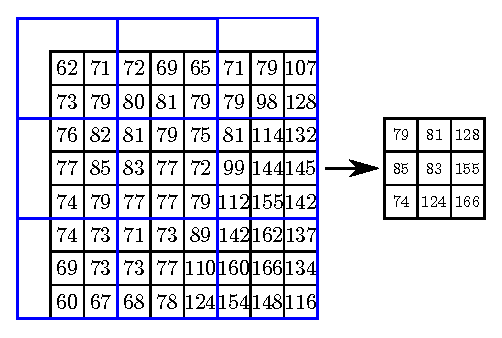
\includegraphics[scale = 0.6]{fig/eps/pooling.eps}
%  \caption{プーリングの例.プーリングサイズ$3\times 3$,ストライド$s=3$,ゼロパディングで最大プーリングを行った場合}
% \end{figure}
% 平均プーリングや最大プーリングなどのプーリングを含む一般性を持った表記として,次のLpプーリング(Lp pooling)がある.
% \begin{eqnarray}
%  u_{ijk} = \left(\frac{1}{H^{2}}\sum_{(p,q) \in P_{ij}}z^{P}_{pqk}\right)^{\frac{1}{P}}
% \end{eqnarray}
% $P=1$で平均プーリング,$P=\infty$で最大プーリングが表現できる.

% \end{frame}


%%%% Caffeで学習を行うまでの流れ %%%%
\begin{frame}\frametitle{Caffeで学習を行うまでの流れ}
独自のデータセットを用いて,Caffeで学習を行うまでの流れを下の図に示す.
\begin{figure}[tb]
  \begin{center}
    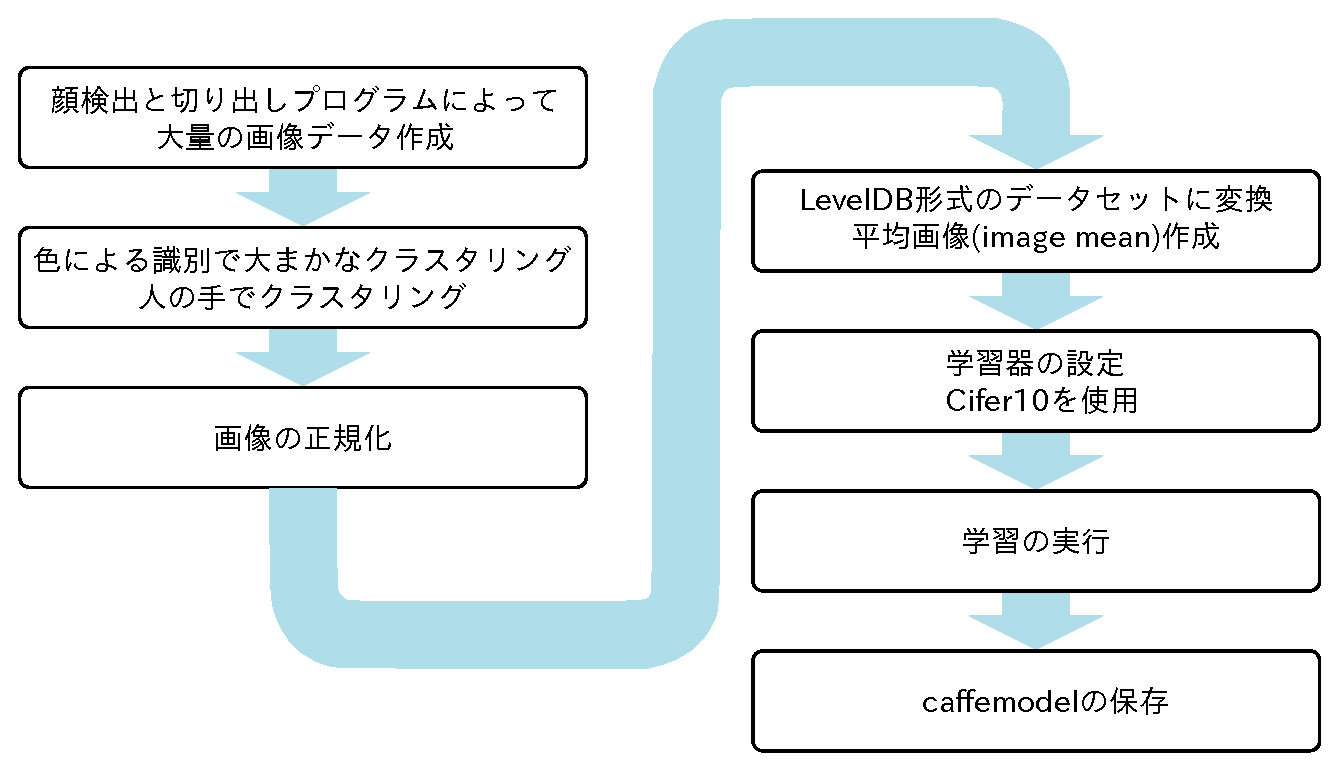
\includegraphics[clip,width=11cm]{./fig/eps/learning_flow.eps}
  \end{center}
\end{figure}

\end{frame}


%%%% Caffeで学習を行うまでの流れ %%%%
\begin{frame}\frametitle{顔検出と大量の画像データ}
前回説明した通りなので今回は省略
\end{frame}

\begin{frame}[fragile]\frametitle{色による大まかなクラスタリング}
OpenCVに実装されているニューラルネットワーク(多層パーセプトロン)を用いて色特徴から大まかにクラスタリング.少量の画像を手動でラベリングして、それを学習.
\begin{lstlisting}[basicstyle=\ttfamily\footnotesize, frame=single, tabsize=2,showtabs,firstnumber=1, numbers=left, breaklines=true]
$ ./cpp/build/train train-labeled.csv train-labeled.csv 
Using training dataset
Training iterations: 908
Results on the testing dataset
 Correct classification: 496 (100%)
 Wrong classifications: 0 (0%)
   0    1   2   3   4   5   6   7   8   9	
0  13   0   0   0   0   0   0   0   0   0   
1  0    12  0   0   0   0   0   0   0   0   
2  0    0   137 0   0   0   0   0   0   0   
3  0    0   0   54  0   0   0   0   0   0   
4  0    0   0   0   11  0   0   0   0   0   
5  0    0   0   0   0   8   0   0   0   0   
6  0    0   0   0   0   0   11  0   0   0   
7  0    0   0   0   0   0   0   19  0   0   
8  0    0   0   0   0   0   0   0   164 0   
9  0    0   0   0   0   0   0   0   0   67
\end{lstlisting}
\end{frame}

\begin{frame}[fragile]\frametitle{最後は人の目}
 \begin{figure}[ht]
  \centering
  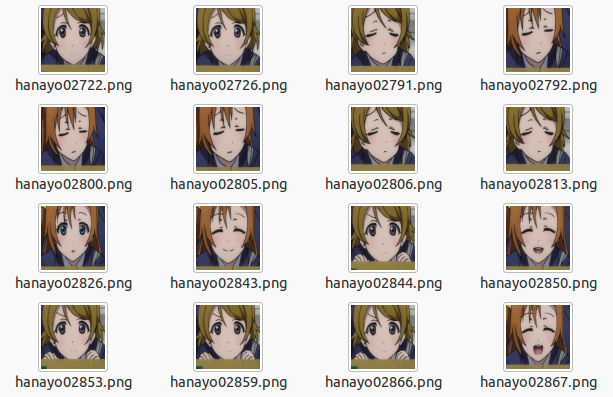
\includegraphics[scale=0.5, bb=0 0 613 397 ]{fig/png/train_result.png}
  \caption{分別結果(正解は「花陽」、「ほのか」が間違い)}
 \end{figure}

\end{frame}

\begin{frame}\frametitle{LevelDB形式のデータセットに変換}
\begin{itemize}
\item 独自のデータセットを用意してCaffeを使って学習させるためには,LevelDB形式と呼ばれる形式のデータセットに変換する必要がある.
\item LevelDB形式はキーバリュー型データストアであり,keyとvalueの紐付けを高速に読み書きできるGoogle製のライブラリである.
\end{itemize}

\begin{exampleblock}{クラス分けした画像ファイルからLevelDBに}
\begin{itemize}
\item この変換は既存のプログラム\cite{SIG2D}を用いて変換を行った.
\item これによって各画像データとラベル番号の紐付けを行う.
\item 全入力画像から9割を訓練データ,1割をテストデータに割り振ることができる.
\end{itemize}
\end{exampleblock}
% \vspace{1cm}
\begin{thebibliography}{99}
  \bibitem{SIG2D} SIG2D,``SIG2D' 14 Proceedings of the 3rd Interdimensional Conference on 2D Information Processing '',\url{http://sig2d.org/publications/},2014.
\end{thebibliography}

\end{frame}

%%%% 学習器の設定 %%%%
\begin{frame}[fragile]\frametitle{学習器の設定}
\begin{itemize}
\item 今回はCifer10の学習モデルをそのまま使用した.
\item ただし最終的な出力の数は学習にかけるラベル数に変更する必要がある.
\item 変更するファイルはcifar10\_quick\_train\_test.prototxtとcifar10\_quick.prototxtである.
\end{itemize}

\begin{lstlisting}[basicstyle=\ttfamily\footnotesize, frame=single, firstnumber=1, numbers=left, breaklines=true]
layers {
  name: "ip2"
  type: INNER_PRODUCT
  bottom: "ip1"
  top: "ip2"
  blobs_lr: 1
  blobs_lr: 2
  inner_product_param {
    num_output: 10      ここを変更
    weight_filler {
\end{lstlisting}
\end{frame}

\begin{frame}[fragile]\frametitle{学習の実行}
\begin{itemize}
\item 以下のコマンドによって学習を実行する.
\item 学習は前回発表したように,GPUを用いて行った.
\item GPUを用いる場合,標準設定がGPUで行うように設定してあるので,設定ファイルの記述を変更する必要はない.
\item CPUのみを用いる場合,cifar10\_full\_solver.prototxtを最後の行にあるsolver\_mode: GPUをCPUに変更する.
\end{itemize}

\begin{lstlisting}[basicstyle=\ttfamily\footnotesize, frame=single, firstnumber=1, numbers=left, breaklines=true]
caffe train --solver examples/cifar10/cifar10_quick_solver.prototxt
\end{lstlisting}

学習が完了すると,cifar10\_quick\_iter\_4000.caffemodelというファイルが生成される.
\end{frame}

%%%% 今後の課題 %%%%
\begin{frame}\frametitle{今後の課題}

\begin{block}{理論研究}
CNNの詳細な調査
\end{block}

\vspace{1cm}
\begin{exampleblock}{プログラミング}
データセットの作成,学習実行結果の評価と過程の可視化
\end{exampleblock}
\end{frame}

% \begin{figure}[t]
%  \begin{minipage}{0.3\hsize}
%   \centering
%   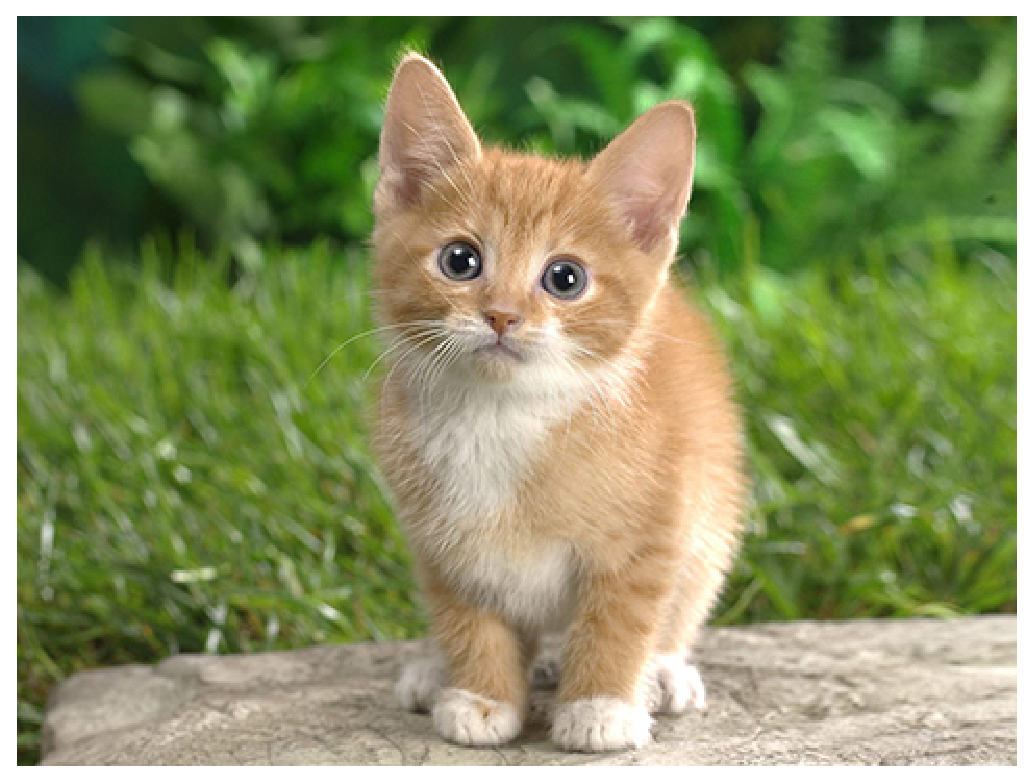
\includegraphics[width=30mm]{./figure/cat.eps}
%   \caption{cat.jpg}
%   \label{sample1}
%  \end{minipage}
%  \begin{minipage}{0.3\hsize}
%   \centering
%   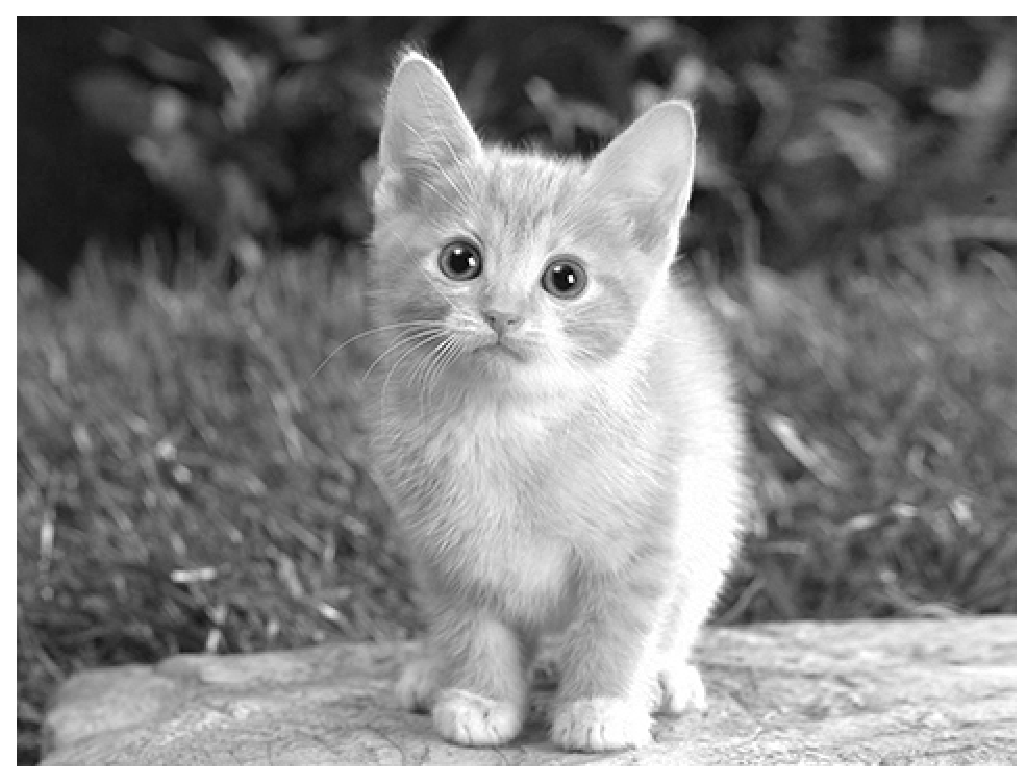
\includegraphics[width=30mm]{./figure/cat_gray.eps}
%   \caption{cat\_gray.jpg}
%   \label{sample2}
%  \end{minipage}
%  \begin{minipage}{0.3\hsize}
%   \centering
%   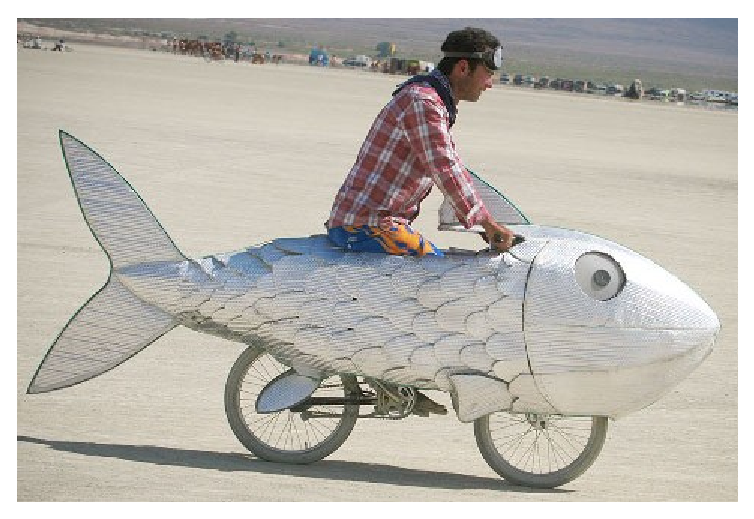
\includegraphics[width=30mm]{./figure/fish-bike.eps}
%   \caption{fish-bike.jpg}
%   \label{sample3}
%  \end{minipage}
% \end{figure}
% \begin{exampleblock}{実行環境}
% \begin{itemize}
%  \item Ubuntu 14.04 LTS
%  \item Intel core i5-4440 3.10GHz$\times$4
%  \item RAM 16GB
% \end{itemize}
% \end{exampleblock}
% \end{frame}


% \section{具体例}

% \begin{frame}\frametitle{定理環境の例}
% \begin{theorem}[Fermat]
% $a^{p-1} \equiv 1 \pmod{p}$
% \end{theorem}
% \pause
% \begin{theorem}[Wilson]
% \begin{equation}
% (p-1)! \equiv 1 \pmod{p}
% \end{equation}
% \end{theorem}
% \end{frame}

% \begin{frame}<1-2>\frametitle{オーバーレイ}
% \onslide*<1>{
% \Large{これは1枚目です}
% }
% \onslide*<2>{
% これは2枚目です
% \begin{theorem}[Euclid]
% There is no largest prime number.
% \end{theorem}
% }
% \end{frame}

% \begin{frame}\frametitle{色もつけれるよ}
%   {\color{red} red}(\alert{alert}),
%   {\color{blue} blue}(\structure{structure}),
%   {\color{green} green},
%   {\color{cyan} cyan},
%   {\color{magenta} magenta},
%   {\color{yellow} yellow},
%   {\color{black} black},
%   {\color{darkgray} darkgray},
%   {\color{gray} gray},
%   {\color{lightgray} lightgray},
%   {\color{orange} orange},
%   {\color{violet} violet},
%   {\color{purple} purple},
%   {\color{brown} brown},
% \end{frame}

% \begin{frame}\frametitle{いろんなブロック}
% \begin{block}{ブロック}
% これは普通のブロックです
% \end{block}

% \begin{alertblock}{警告ブロック}
% 警告!これは警告ブロックだ!
% \end{alertblock}

% \begin{exampleblock}{例ブロック}
% 例えば、こんなブロックです。
% \end{exampleblock}
% \end{frame}

% \begin{frame}<1-2>\frametitle{画像も貼れるよ}
% \onslide*<1>{
% このように画像を貼れるよ
% %\begin{figure}[htb]
% %\centering
% %\includegraphics[width=12cm,clip]{dummygraph.pdf}
% %\caption{$f(x)=e^{-\frac{x}{10}}\sin(x)$}
% %\end{figure}%
% }
% \onslide*<2>{
% 画像や表は各自用意してね
% %\begin{figure}[htb]
% %\centering
% %\includegraphics[width=8cm,clip]{sym4.pdf}
% %\caption{Cayley graph of $\mathfrak{S}_{4}$}
% %\end{figure}%
% }
% \end{frame}

% \begin{frame}\frametitle{まとめ}
% \LARGE{大事なのは中身です!}
% \end{frame}

% \begin{frame}\frametitle{}
% {\Large ありがとうございました}
% \end{frame}
% \appendix

\newcounter{finalframe}
\setcounter{finalframe}{\value{framenumber}}

% \begin{frame}[containsverbatim]\frametitle{dvipngの使い方(1)}
% \begin{block}{この様なファイルを用意する}
% \tiny{
% \begin{verbatim*}
% \documentclass[43pt]{jsarticle}
% \usepackage{amsmath}
% \usepackage{lmodern}
% \pagestyle{empty}
% \begin{document}
% \begin{equation*}
% \sum_{k=0}^{\infty} \frac{(2k)!}{2^{2k}(k!)^2} \frac{1}{2k+1}=\frac{\pi}{2}
% \end{equation*}
% \end{document}
% \end{verbatim*}
% }
% \end{block}
% \end{frame}

% \begin{frame}[containsverbatim]\frametitle{dvipngの使い方(2)}
% \begin{block}{使い方(コマンドライン)}
% \scriptsize{
% \begin{verbatim*}
% latex dvipng-sample.tex
% dvipng dvipng-sample.dvi -T tight -bd 1000
% \end{verbatim*}
% }
% \end{block}
% \end{frame}
\setcounter{framenumber}{\value{finalframe}}
\end{document}